\documentclass[slidestop,compress,mathserif]{beamer}
\usetheme{Frankfurt}
\usecolortheme{seagull}

% Load packages
\usepackage{alltt}
\usepackage{verbatim}
\usepackage{geometry}                % See geometry.pdf to learn the layout options. There are lots.
\usepackage{graphicx}
\usepackage{amssymb}
\usepackage{amsmath}
\usepackage{epstopdf}
\usepackage{verbatim}
%\usepackage{musixtex}
%\usepackage{xymtexps}
\usepackage{feynmp}

%\usepackage{pgfpages}
%\pgfpagesuselayout{4 on 1}[letterpaper,landscape,border shrink=5mm]

\DeclareGraphicsRule{.tif}{png}{.png}{`convert #1 `dirname #1`/`basename #1 .tif`.png}


% Title 
% Note: [short title]{long title}, [short author(s) name]{long author(s) name}
\title{Intro to LaTeX, Part II: \\Math, BibTeX, and Customization}
\subtitle{}
\author{David Diez} 
\institute{OpenIntro \\ \href{http://www.openintro.org}{openintro.org}}
\date{}

\begin{document}
\definecolor{highlight}{rgb}{.7,.1,.1}
\definecolor{command}{rgb}{.1,.1,.9}
\definecolor{comment}{rgb}{1,0,0}
\definecolor{braces}{rgb}{0,0.5,0}
\newenvironment{act}[1]{{\color{command}#1}}{}
\newcommand{\lcom}[1]{{\color{command}$\backslash$#1}}
\newcommand{\larg}[1]{{\color{braces}$\{${\color{black}#1}$\}$}}
\newcommand{\mathText}[1]{{\color{braces}\${\color{black}#1}\$}}


\frame{ \titlepage }

\begin{frame}
  \frametitle{Outline}
  \begin{itemize}
  \item Mathematics in LaTeX
  \item BibTeX: bibliographies in LaTeX
  \item Building your own commands and environments
  \item Miscellaneous tips
  \end{itemize}
\end{frame}

\begin{frame}  \frametitle{Guide to LaTeX}
The book \textit{Guide to LaTeX} offers a very nice introduction, and we will closely follow some of the examples in these chapters in this class:
\begin{itemize}
\item[7] math
\item[11,12] BibTeX, and
\item[10] custom commands and environments.
\end{itemize}
%If you are looking for a LaTeX resource, \textit{Guide to LaTeX} is a good choice.
\end{frame}

\part{}


%READ ME
% two new commands were created to ease LaTeX command appearance.
%    use \lcom{command} to print a command, which includes coloring and the backslash
%    use \larg{argument} to print an argument in green braces
%    use \mathText{math text} to print an argument with two green $ around it
% additionally, combine the commands:
%    \mathText{\lcom{alpha}}
%    instead of 
%    {\color{braces}\$}\texttt{\color{command}$\backslash$alpha}\texttt{\color{braces}\$}

\section[Math]{Math}

\subsection[Mathematics]{Mathematics}
\begin{frame} \frametitle{Math in LaTeX}
We will cover several aspects of the mathematics environments offered in LaTeX.
\begin{itemize}
\item Basic mathematics in text
\item Different equation environments
\item Mathematical symbols
\item Mathematical expressions
\item Accenting and modifying text
\item Automatic sizing of bracket symbols
\item Text in mathematical equations
\item Arrays and matrices
\end{itemize}
\end{frame}

\subsection[Inserting math]{Inserting math}
\begin{frame} \frametitle{Inserting math into text}
LaTeX makes it easy to add Greek letters like $\alpha$, $\zeta$,
$\mu$, etc. into text. In the same way, equations can be added
easily as well: $y=x^3$, $\sum z^j$, $x_1+\cdots+x_n$.
\begin{center}
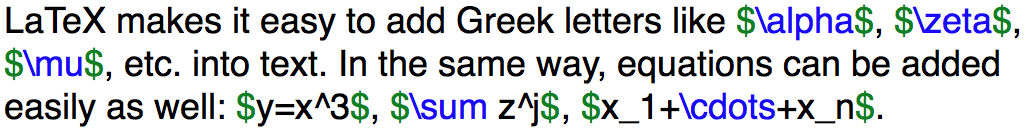
\includegraphics[height=0.47in]{math/mathInText}
\end{center}
The {\color{braces}\$} signs tell LaTeX when to switch into or out of math model. For instance, to create $\alpha$ above, type \mathText{\lcom{alpha}}. %{\color{braces}\$}\texttt{\color{command}$\backslash$alpha}\texttt{\color{braces}\$}.
\vspace{5mm} \\
How can we create $\beta$?
\end{frame}

\begin{frame} \frametitle{Equation array}
Some equations are long and should be on their on lines. In such a case, use the \texttt{\color{highlight}eqnarray} or \texttt{\color{highlight}eqnarray$^*$} environment:
\begin{center}
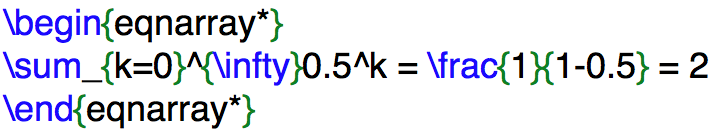
\includegraphics[height=0.4in]{math/eqnarrayStar}
\end{center}
The result in LaTeX for \texttt{\color{highlight}eqnarray$^*$}:
\begin{eqnarray*}
\sum_{k=0}^{\infty}0.5^k = \frac{1}{1-0.5} = 2
\end{eqnarray*}
\end{frame}

\begin{frame} \frametitle{Equation referencing}
Just like tables and figures, equations can be referenced. Use \texttt{\color{highlight}eqnarray} (no asterisk) to add an equation number:
\begin{eqnarray}
\sum_{k=0}^{\infty}0.5^k = \frac{1}{1-0.5} = 2
\end{eqnarray}
\texttt{\color{command}$\backslash$label}\texttt{\color{braces}\{}\texttt{powerSeries}\texttt{\color{braces}\}} can be put inside the equation array and then be referenced via \texttt{\color{command}$\backslash$ref}\texttt{\color{braces}\{}\texttt{powerSeries}\texttt{\color{braces}\}}.
\begin{center}
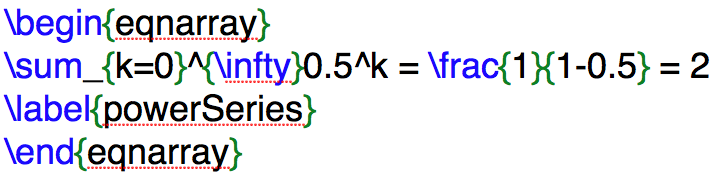
\includegraphics[height=0.6in]{math/eqnarray}
\end{center}
\end{frame}

\begin{frame} \frametitle{Aligned equations}
Another environment, \texttt{\color{highlight}align} (and \texttt{\color{highlight}align$^*$}) are handy for aligning multiline equations.
\begin{center}
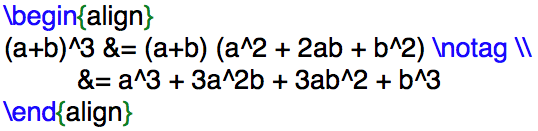
\includegraphics[height=14mm]{math/align}
\end{center}
Result:
\begin{align}
(a+b)^3 &= (a+b) (a^2 + 2ab + b^2) \notag \\
	      &= a^3 + 3a^2b + 3ab^2 + b^3
\end{align}
The \texttt{\color{command}$\backslash\backslash$} command creates a line break. The command \texttt{\color{command}$\backslash$notag} was used to suppress the equation number of the first line, which requires the \texttt{\color{highlight}amsmath} package. (Q: We have an equation number. What should I have included in the code?)
\end{frame}

\begin{frame} \frametitle{Multiple alignments}
The \texttt{\color{highlight}align} environment permits several alignments:
\begin{center}
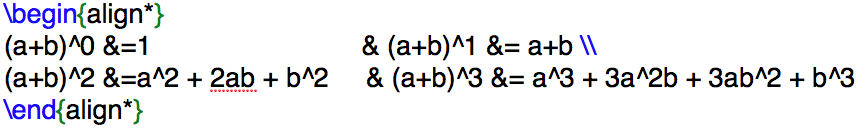
\includegraphics[height=14mm]{math/alignMany}
\end{center}
outputs
\begin{align*}
(a+b)^0 &=1                            & (a+b)^1 &= a+b \\
(a+b)^2 &=a^2 + 2ab + b^2     & (a+b)^3 &= a^3 + 3a^2b + 3ab^2 + b^3
\end{align*}
%The \texttt{\color{command}$\backslash\backslash$} command creates a line break. The command \texttt{\color{command}$\backslash$notag} was used to suppress the equation number of the first line (package \texttt{\color{highlight}amsmath} required).
%\texttt{\color{command}$\backslash$label}\texttt{\color{braces}\{}\texttt{powerSeries}\texttt{\color{braces}\}} can be put inside the equation array and then be referenced via \texttt{\color{command}$\backslash$ref}\texttt{\color{braces}\{}\texttt{powerSeries}\texttt{\color{braces}\}}.
\end{frame}

\subsection[Mathematics and symbols]{Mathematics and symbols}

\begin{frame} \frametitle{Mathematics and symbols}
It is a little difficult to learn all the math syntax and a good help source is the LaTeX and Matrix Panels:
\begin{center}
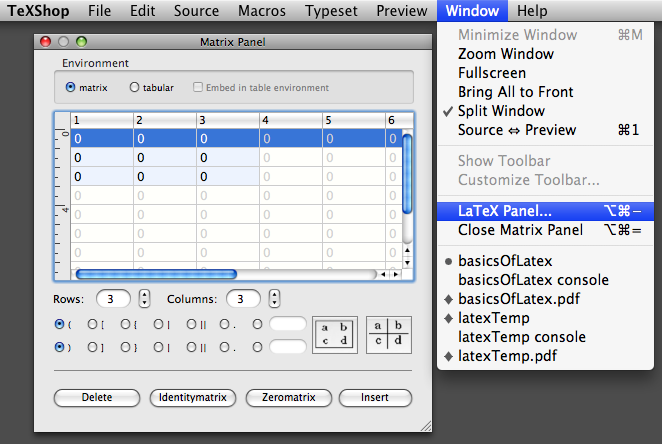
\includegraphics[height=1.5in]{math/panels}
\end{center}
The Matrix Panel is especially useful since matrices can require a lot of writing. The LaTeX panel is handy as a quick reference.
\end{frame}

\begin{frame} \frametitle{Some symbols}
Here is a very small subset of the symbols available in LaTeX.
%\begin{center}
\begin{tabular}{rl p{4mm} rl p{4mm} rl}
$\leftarrow$ & {\color{braces}\${\color{command}$\backslash$leftarrow}\$} &&
$\Leftarrow$ & {\color{braces}\${\color{command}$\backslash$Leftarrow}\$} && 
$\leftrightarrow$ & {\color{braces}\${\color{command}$\backslash$leftrightarrow}\$} \\
$\geq$ & {\color{braces}\${\color{command}$\backslash$geq}\$} &&
$\neq$ & {\color{braces}\${\color{command}$\backslash$neq}\$} &&
$\not\in$ & {\color{braces}\${\color{command}$\backslash$not$\backslash$in}\$} \\
$\partial$ & {\color{braces}\${\color{command}$\backslash$partial}\$} &&
$\oint$ & {\color{braces}\${\color{command}$\backslash$oint}\$} &&
$\nabla$ & {\color{braces}\${\color{command}$\backslash$nabla}\$} \\
$\bigcap$ & {\color{braces}\${\color{command}$\backslash$bigcap}\$} &&
$\bigcup$ & {\color{braces}\${\color{command}$\backslash$bigcup}\$} &&
$\cap$ & {\color{braces}\${\color{command}$\backslash$cap}\$} \\
$\subset$ & {\color{braces}\${\color{command}$\backslash$subset}\$} &&
$\supseteq$ & {\color{braces}\${\color{command}$\backslash$supseteq}\$} &&
$\not\supseteq$ & {\color{braces}\${\color{command}$\backslash$not$\backslash$supseteq}\$} \\
$\bigodot$ & {\color{braces}\${\color{command}$\backslash$bigodot}\$} &&
$\bigotimes$ & {\color{braces}\${\color{command}$\backslash$bigotimes}\$} &&
$\oplus$ & {\color{braces}\${\color{command}$\backslash$oplus}\$} \\
$\clubsuit$ & {\color{braces}\${\color{command}$\backslash$clubsuit}\$} &&
$\perp$ & {\color{braces}\${\color{command}$\backslash$perp}\$} &&
$\vdash$ & {\color{braces}\${\color{command}$\backslash$vdash}\$} \\
\end{tabular}
%\end{center}
For a searchable PDF with thousands of symbols, see
\begin{itemize}
\item[] {\small\color{highlight}www.ctan.org/tex-archive/info/symbols/comprehensive/symbols-a4.pdf}
\end{itemize}
Also see the LaTeX Panel (under the menu item {\color{highlight}Window}).
\end{frame}

\begin{frame} \frametitle{Character modifications}
Text and symbols in math mode can also be modified.
\begin{center}
\begin{tabular}{rl p{4mm} rl p{4mm} rl}
\hline
\multicolumn{3}{l}{Regular} & {Modified} &&& {Accents} & \\
\hline
{\color{braces}\${\color{black}R}\$} & $R$ &&
{\color{braces}\${\color{command}$\backslash$mathbb}$\{${\color{black}R}$\}$\$} & $\mathbb{R}$ &&
{\color{braces}\${\color{command}$\backslash$tilde}$\{${\color{black}R}$\}$\$} & $\tilde{R}$ \\
{\color{braces}\${\color{black}A}\$} & $A$ &&
{\color{braces}\${\color{command}$\backslash$mathcal}$\{${\color{black}A}$\}$\$} & $\mathcal{A}$ &&
{\color{braces}\${\color{command}$\backslash$widetilde}$\{${\color{black}A}$\}$\$} & $\widetilde{A}$ \\
{\color{braces}\${\color{black}x}\$} & $x$ &&
{\color{braces}\${\color{command}$\backslash$mathbf}$\{${\color{black}x}$\}$\$} & $\mathbf{x}$ &&
{\color{braces}\${\color{command}$\backslash$bar}$\{${\color{black}x}$\}$\$} & $\bar{x}$ \\
{\color{braces}\${\color{black}p}\$} & $p$ &&
{\color{braces}\${\color{command}$\backslash$mathit}$\{${\color{black}p}$\}$\$} & $\mathit{p}$ &&
{\color{braces}\${\color{command}$\backslash$hat}$\{${\color{black}p}$\}$\$} & $\hat{p}$ \\
{\color{braces}\${\color{black}X}\$} & $X$ &&
{\color{braces}\${\color{command}$\backslash$mathrm}$\{${\color{black}X}$\}$\$} & $\mathrm{X}$ &&
{\color{braces}\${\color{command}$\backslash$widehat}$\{${\color{black}X}$\}$\$} & $\widehat{X}$ \\
\hline
\end{tabular}
\end{center}
Two other accents: $\dot{x}$ and $\ddot{x}$ via {\color{braces}\${\color{command}$\backslash$dot}$\{${\color{black}x}$\}$\$} and {\color{braces}\${\color{command}$\backslash$ddot}$\{${\color{black}x}$\}$\$}.
\end{frame}

\begin{frame} \frametitle{Subscripts and exponents}
We can create subscripts (e.g. $x_1$) and superscripts (e.g. $3^2$):
\begin{center}

\includegraphics[height=8mm]{math/subSuperscript}
\end{center}
When the subscript is a single character, then it is acceptable to omit the curly braces. That is, the following is equally acceptable for the text above:
\begin{center}

\includegraphics[height=8mm]{math/subSuperscriptNoBraces}
\end{center}
If more than one character is in the sub/superscript, braces are necessary to avoid problems: {\color{braces}\${\color{black}2\textbf{\_}10}\$} outputs $2_10$. Sub and superscripts can be used simultaneously: $x_{ij}^2$.
\end{frame}

\begin{frame} \frametitle{Fractions and roots}
We can easily create fractions such as $\frac{2+3}{4+5} = \frac{5}{9}$ or roots such as $\sqrt{81}=9$ and $\sqrt[4]{81} = 3$.
\begin{center}
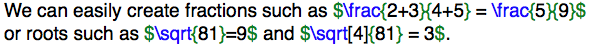
\includegraphics[height=7mm]{math/fracRoots}
\end{center}
And we can combine them as well:
$\frac{\sqrt{4} + 3}{\sqrt{16} + 5} = \frac{5}{9}$.
\begin{center}
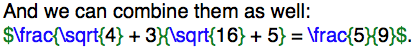
\includegraphics[height=7mm]{math/fracRootsCombined}
\end{center}
\end{frame}

\begin{frame} \frametitle{Sums and integrals}
We can also create sums and integrals:
\begin{center}
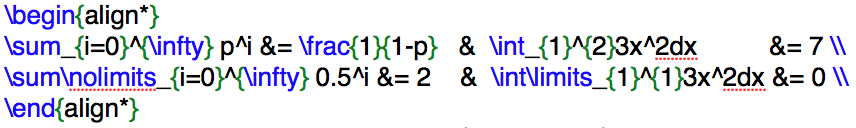
\includegraphics[height=14mm]{math/sumIntegral}
\end{center}
which results in
\begin{align*}
\sum_{i=0}^{\infty} p^i &= \frac{1}{1-p}   &  \int_{1}^{2}3x^2dx          &= 7 \\
\sum\nolimits_{i=0}^{\infty} 0.5^i &= 2    &  \int\limits_{1}^{1}3x^2dx &= 0
\end{align*}
The commands \texttt{\color{command}$\backslash$nolimits} and \texttt{\color{command}$\backslash$limits} can be used to override the default displays of limits in LaTeX.
\end{frame}

\begin{frame} \frametitle{Practice}
Produce the following result using the \texttt{\color{highlight}eqnarray$^*$} environment:
\begin{center}
   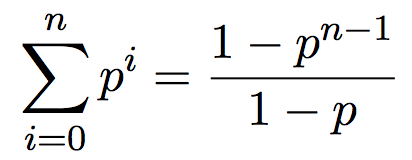
\includegraphics[height=0.6in]{math/tryIt3}
\end{center}
Some examples may be utilized in \texttt{\color{highlight}latexTemp.tex}.
\end{frame}

\subsection[Final items]{Final items}
\begin{frame} \frametitle{Sizing of Brackets}
A small problem with bracket sizes is shown in the left equation, and this problem is fixed on the right.
\begin{align*}
   (\frac{2+3}{4+5}) &&& \left(\frac{2+3}{4+5}\right)
\end{align*}
The coding for the expressions above 
\begin{center}
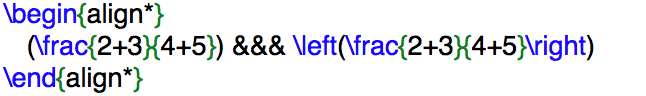
\includegraphics[height=9mm]{math/fixingParentheses}
\end{center}
Generally we can use {\color{command}$\backslash$left\color{black}(}, {\color{command}$\backslash$left\color{black}[}, {\color{command}$\backslash$left\color{black}$|$}, and {\color{command}$\backslash$left$\backslash\{$} and their corresponding right brackets to create automatically sized brackets. These commands \emph{must} be inside one of the equations environments and the left and right brackets must always be balanced.
\end{frame}

\begin{frame} \frametitle{Matrices}
Matrices also can be made in LaTeX:
\begin{eqnarray*}
\left(\begin{array}{ccc} 4 & 1 & 19 \\ 3 & 8 & 8\end{array}\right)
\end{eqnarray*}
The code:
\begin{center}
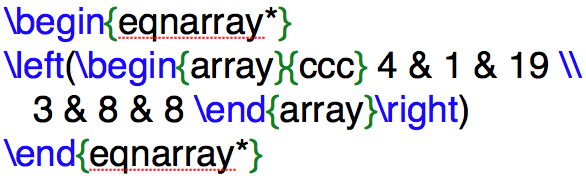
\includegraphics[height=0.6in]{math/array}
\end{center}
The syntax for an \texttt{\color{highlight}array} is the same as for \texttt{\color{highlight}tabular} (a table).
\end{frame}

\begin{frame} \frametitle{Space and stacking}
Space can be added in equations using {\color{command}$\backslash$quad}, and expressions can be stacked via {\color{command}$\backslash$stackrel}:

\vspace{1mm}

\begin{itemize}
\item[] {\color{command}$\backslash$begin}{\color{braces}$\{${\color{black}eqnarray$^*$}$\}$}
\item[] \hspace{2mm} E(X+Y)
	{\color{command}$\backslash$stackrel\color{braces}$\{${\color{black}indep.}$\}\{${\color{black}=}$\}$}
	E(X) + E(Y)
\item[] \hspace{5mm} {\color{command}$\backslash$quad$\backslash$quad}
\item[] \hspace{5mm} Var(X+Y)
	{\color{command}$\backslash$stackrel\color{braces}$\{${\color{black}indep.}$\}\{${\color{black}=}$\}$}
	Var(X) + Var(Y)
\item[] {\color{command}$\backslash$end}{\color{braces}$\{${\color{black}eqnarray$^*$}$\}$}
\end{itemize}

\vspace{1mm}

produces
\begin{eqnarray*}
E(X+Y) \stackrel{indep.}{=} E(X) + E(Y) \quad\quad Var(X+Y) \stackrel{indep.}{=} Var(X) + Var(Y)
\end{eqnarray*}
\end{frame}




\section[BibTeX Overview]{BibTeX Overview}

\begin{frame}  \frametitle{Why use BibTeX?}
	There are a number of very good reasons to use BibTeX instead of manual creation of bibliographies.
	\begin{itemize}
		\item Automatic creation of bibliographies.
		\item Easily change bibliographic styles.
		\item Identification of missing sources referenced in text.
	\end{itemize}
\end{frame}

\begin{frame}  \frametitle{How BibTeX works}
	There are three steps that LaTeX and BibTeX take to make a bibliography.
	\begin{itemize}
		\item When you typeset a document with citations (e.g. {\color{command}$\backslash$cite{\color{braces}$\{$}{\color{black}zotova}{\color{braces}$\}$}}), LaTeX makes note of each citation.
		\item BibTeX takes this list and looks for each reference in a database of publications.
		\item Then we tell LaTeX to make the bibliography of all of those publications it found that we referenced.
	\end{itemize}
	The most time consuming part is initially building the database. After that, you can reference this same database over and over again and BibTeX becomes a breeze.
\end{frame}

\begin{frame}  \frametitle{BibTeX material}
	\begin{itemize}
		\item Creating your database
		\item Citing a reference
		\item Typesetting with BibTeX
		\item Building style files
	\end{itemize}
\end{frame}

\section[Building the database]{Building the database}

\begin{frame}  \frametitle{Sample reference entry}
	We want to create a reference, similar to the following, for each of the item we want to cite.
	
	\vspace{7mm}
	
	@article$\{\overbrace{\text{zotova}}^{label}$, \\
	\hspace{3mm}	Author = $\{$Elena Zotova and Charles D Woody and Ehud Gruen$\}$, \\
	\hspace{3mm}	Journal = $\{$Brain Research$\}$, \\
	\hspace{3mm}	Pages = $\{$66-78$\}$, \\
	\hspace{3mm}	Title = $\{$Multiple representations ... [etc etc].$\}$, \\
	\hspace{3mm}	Volume = $\{$868$\}$, \\
	\hspace{3mm}	Year = $\{$2000$\}\}$ \\
\end{frame}

\begin{frame}  \frametitle{Make up of a reference}
	Each reference needs a publication type (e.g. article, book), and each reference includes many fields. For instance, the following are \textbf{required} and \textit{optional} fields of an article entry.
	\begin{center}
		\begin{tabular}{lllrr}
			\multicolumn{5}{l}{\textbf{label}: The reference label.} \\
			\textbf{Author} & \textbf{Journal} & \textbf{Title} & \hspace{5mm} & \\
			\textbf{Year} & \textit{Volume} & \textit{Number} \\
			\textit{Pages} & \textit{Month} & \textit{Note}
		\end{tabular}
	\end{center}
	A formal list of the available publication types and also which items are required and optional for each type, see
	\begin{itemize}
		\item[]\color{highlight}http://www.image.ufl.edu/help/latex/entry\_bibtex.shtml
	\end{itemize}
\end{frame}

\begin{frame}  \frametitle{An alternative}
	If you don't want to build your data base up in such a bare-bones manner, you might try
	\begin{itemize}
		\item BibDesk: Macs.
		\item JabRef: Macs, PCs, Linux.
	\end{itemize}
	Both of these programs are free and available online. Others exist, and I have only personally used BibDesk.
\end{frame}

\begin{frame}  \frametitle{If you do manage your own...}
	Some things you should know if you do not use a program manager:
	\begin{itemize}
		\item Always include a label, which is how LaTeX identifies the entry.
		\item The entry (publication) type and field names are NOT cap-sensitive.
		\item Enclose the text for each field (e.g. the author names) in curly braces.
		\item You can add extra fields that are not listed and these will be ignored (e.g. if you add an Abstract field to a reference, BibTeX will just ignore it).
	\end{itemize}
\end{frame}

\begin{frame}  \frametitle{Special cases}
	Giving author names in a non-ambiguous form is sometimes difficult.
	\begin{itemize}
		\item Always type names as $\{$Given Names Surnames$\}$ or $\{$Surname, Given Names$\}$.
		\item Anything enclosed in braces will be treated as a single item (e.g. Author = {\color{braces}$\{${\color{black}Maria} $\{${\color{black}San Martino}$\}\}$}).
		\item If there is more than one author, separate each author name by the word \textit{and}. If \textit{and} is part of someone's name, enclose their entire name in braces.
		\item You may add accents (e.g. G$\ddot{\text{o}}$del via \texttt{G$\{\backslash$"o$\}$del}).
	\end{itemize}
	Many other nuances exist. If you encounter a peculiar name, do a little online searching to see how best to put it into the data base.
\end{frame}

\begin{frame}  \frametitle{Abbreviating journal names}
	Sometimes you don't want your entry to include the entire journal name. To shorten it, use the \textit{string} entry type:
	\begin{itemize}
		\item[] @string$\{$JSS = $\{$Journal of Statistical Software$\}\}$
	\end{itemize}
	These string entries must be defined in the database above where they are used.
\end{frame}

\subsection{Citing a reference}

\begin{frame}  \frametitle{Citing a reference}
	There are four commands that can be used.
	\begin{itemize}
		\item {\color{command}$\backslash$cite\color{braces}$\{${\color{black}labelName}$\}$} [referenceNumber], e.g. [1].
		\item {\color{command}$\backslash$citet\color{braces}$\{${\color{black}labelName}$\}$} Surname (year), e.g. Zotova et al. (2000).
		\item {\color{command}$\backslash$citep\color{braces}$\{${\color{black}labelName}$\}$} (Surname, year), e.g. (Zotova et al., 2000).
		\item {\color{command}$\backslash$nocite\color{braces}$\{${\color{black}labelName}$\}$} Not cited but will show up in bibliography.
	\end{itemize}
	The first and last work with the \texttt{\color{highlight}uclathes} class. The second two are used in the \texttt{\color{highlight}natbib} package (highly recommended for non-thesis papers).
\end{frame}

\begin{frame}  \frametitle{Other commands in your document}
	The following two lines of code must be inserted at the place where the bibliography is to be added:
	\begin{itemize}
		\item[] {\color{command}$\backslash$bibliographystyle\color{braces}$\{${\color{black}yourStyle}$\}$}
		\item[] {\color{command}$\backslash$bibliography\color{braces}$\{${\color{black}databaseName}$\}$}
	\end{itemize}
	The style command can be moved higher (it doesn't matter). If you use the \texttt{\color{highlight}natbib} package, then you must add it with the other packages:
	\begin{itemize}
		\item[] {\color{command}$\backslash$usepackage\color{braces}$\{${\color{black}natbib}$\}$}
	\end{itemize}
	I have not gotten this package to work with the UCLA thesis template.
\end{frame}

\subsection{Typesetting}

\begin{frame}  \frametitle{Making the bibliography}
	If you have made your reference database, made citations, and inserted the bibliography commands in your text, then you are ready to create the bibliography. In TeXShop, there are a few simple steps to finish:
	\begin{itemize}
		\item Typeset your LaTeX document as usual.
		\item Change the Typesetting option from LaTeX to BibTeX:
		
		\vspace{1mm}
		
		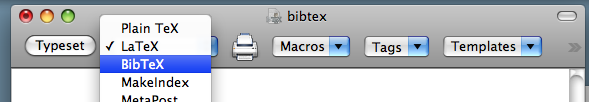
\includegraphics[height=15mm]{bibtex/bibtexTypeset}\hspace{4mm}{}
		
		\item Typeset again with BibTeX.
		\item Return the Typesetting option back to LaTeX and compile \textbf{twice} more.
	\end{itemize}
\end{frame}

\subsection{Building your own style file (the easy way)}

\begin{frame}  \frametitle{Building a style file}
	One of the big benefits of BibTeX is the ability to quickly change the bibliography style and within-text citations. To do this, we use the program {\color{highlight}custom-bib}. Download it at
	\begin{itemize}\small 
		\item[] \color{highlight} http://www.ctan.org/tex-archive/help/Catalogue/entries/custom-bib.html
	\end{itemize}
	custom-bib has been included in the {\color{highlight}latexTemp} zip file from the first class.
\end{frame}

\begin{frame}  \frametitle{Building a style file}
	Open \texttt{latexTemp} $>$ \texttt{custom-bib}, and open the \texttt{\color{highlight}makebst.tex} file. To run the program,
	\begin{itemize}
		\item[(1)] Open the file and typeset it.
		\item[(2)] Type \texttt{YES} to the first question to get extra directions.
		\item[(3)] Choose an appropriate file name (no need to add the extension).
		\item[(4)] Answer each of the style questions.
		\item[(5)] For the last question, \textit{Finished!! ...  Shall I now run this batch job? (NO)}, type \texttt{YES}.
	\end{itemize}
	Find and copy the file you named in step (3) with extension \texttt{.bst}. Put it in the folder with whatever files for which you will make a bibliography with this style or in your bibliography folder (however you reference it in your LaTeX document).
\end{frame}

\section{Practice}

\begin{frame}  \frametitle{Practice}
	Open the \texttt{\color{highlight}latexTemp.tex} file and go to the last section. Add a bibliography reference of {\color{command}$\backslash$citet}{\color{braces}$\{${\color{black}victor}$\}$}. Also add a reference with {\color{command}$\backslash$citep}{\color{braces}$\{${\color{black}victor}$\}$} and typeset (all four steps). What is the difference between your references? How would you use each in a paper?\end{frame}




\section[Customization]{Customization}

\subsection[To be covered]{To be covered}

\begin{frame}  \frametitle{Custom command material}
\begin{itemize}
\item Counters
\item Creating commands
\item Creating environments
\end{itemize}
\end{frame}

\subsection[Counters]{Counters}

\begin{frame}  \frametitle{Existing counters}
LaTeX uses counters (variables) to keep proper numbering. 
\begin{itemize}
\item The following are counters used by LaTeX: \texttt{\color{highlight}part}, \texttt{\color{highlight}chapter}, \texttt{\color{highlight}section}, \texttt{\color{highlight}subsection}, \texttt{\color{highlight}subsubsection}, \texttt{\color{highlight}page}, \texttt{\color{highlight}footnote}, \texttt{\color{highlight}equation}, \texttt{\color{highlight}figure}, and \texttt{\color{highlight}table}. These counters correspond to their corresponding commands.
\item Other counters are used for each level of enumerate: \texttt{\color{highlight}enumi}, \texttt{\color{highlight}enumii}, \texttt{\color{highlight}enumiii}, \texttt{\color{highlight}enumiv}.
\item A few other LaTeX counters: \texttt{\color{highlight}paragraph}, \texttt{\color{highlight}subparagraph}, \texttt{\color{highlight}mpfootnote}.
\end{itemize}
\end{frame}

\begin{frame}  \frametitle{Create new counters}
We may want to create our own counters for our own purposes. Maybe we have examples that we want numbered.
\begin{itemize}
\item[] {\color{command}$\backslash$newcounter\color{braces}$\{${\color{black}counterName}$\}$\color{black}[inCounter]}
\end{itemize}
This creates a new counter called \texttt{counterName}. The \texttt{inCounter} argument $+$ brackets are optional and an \texttt{inCounter} is used to reset \texttt{counterName} whenever \texttt{inCounter} increments (e.g. \texttt{subsection} has ``inCounter'' \texttt{section}).
\end{frame}

\begin{frame}  \frametitle{Modifying}
We can modify existing or new counters.
\begin{itemize}
\item[] {\color{command}$\backslash$setcounter\color{braces}$\{${\color{black}counter}$\}\{${\color{black}n}$\}$}
\item[] {\color{command}$\backslash$addtocounter\color{braces}$\{${\color{black}counter}$\}\{${\color{black}n}$\}$}
\item[] {\color{command}$\backslash$stepcounter\color{braces}$\{${\color{black}counter}$\}$}
\item[] {\color{command}$\backslash$refstepcounter\color{braces}$\{${\color{black}counter}$\}$}
\end{itemize}
The {\color{command}$\backslash$refstepcounter} command lets us reference our counter value if we follow it with a {\color{command}$\backslash$label}.
\end{frame}

\begin{frame}  \frametitle{Printing}
So we can create, modify, and reference counters. However, we also need to print counters in the document. We do so by calling the counter with one of the following commands:
\newcounter{temp}
\setcounter{temp}{4}
\begin{itemize}
\item[] {\color{command}$\backslash$arabic}{\color{braces}$\{${\color{black}chapter}$\}$} (\arabic{temp}, Arabic number)
\item[] {\color{command}$\backslash$Roman} (\Roman{temp}, uppercase Roman numeral)
\item[] {\color{command}$\backslash$roman} (\roman{temp}, lowercase Roman numeral)
\item[] {\color{command}$\backslash$Alph} (\Alph{temp}, capital letter)
\item[] {\color{command}$\backslash$alph} (\alph{temp}, lowercase letter)
\item[] {\color{command}$\backslash$fnsymbol} (\fnsymbol{temp}, footnote symbol)
\end{itemize}
We will put counters to use in our custom commands and environments.
\end{frame}

\subsection[Commands]{Commands}

\begin{frame}  \frametitle{Simple command}
\newcommand{\xvec}{x_1, \ldots, x_n}
Common statements, like $x_1, ..., x_n$ can be abbreviated using a new command.
\begin{itemize}
\item[] {\color{command}$\backslash$newcommand\color{braces}$\{${\color{command}$\backslash$xvec}$\}\{${\color{black}x\_1,{\color{command}$\backslash$dots},x\_n}$\}$}
\end{itemize}
Inserting this command and then typing (later in the document) {\color{braces}\$\color{command}$\backslash$xvec\color{braces}\$}, we get $\xvec$. If we forgot the dollar signs, we would be in trouble. We can resolve this by using an extra command:
\begin{itemize}
\item[] {\color{command}$\backslash$newcommand\color{braces}$\{${\color{command}$\backslash$xvec}$\}\{${\color{command}$\backslash$ensuremath{\color{braces}$\{$}{\color{black}x\_1,{\color{command}$\backslash$dots},x\_n}}$\}$ $\}$}
\end{itemize}
In the second definition, we left an extra space at the end, which helps prevent spacing problems. More elegant solution is to use the {\color{highlight}xspace} package (see \textit{Guide to LaTeX}, page 186).
\end{frame}

\newcommand{\subvec}[2]{\ensuremath{#1_{1}, \ldots, #1_{#2}} }
\begin{frame}  \frametitle{Command with arguments}
If we want to generalize our command, we add two arguments
\begin{itemize}
\item[] \hspace{-1mm}{\color{command}$\backslash$newcommand\color{braces}$\{${\color{command}$\backslash$subvec}$\}${\color{black}[2]}$\{${\color{command}$\backslash$ensuremath{\color{braces}$\{$}{\color{black}\#1\_1,{\color{command}$\backslash$dots},\#1\_{\color{braces}$\{$}\#2{\color{braces}$\}$}}}$\}$ $\}$}
\end{itemize}
We can create \subvec{y}{m} from {\color{command}$\backslash$subvec\color{braces}$\{${\color{black}y}$\}\{${\color{black}m}$\}$}.

\vspace{7mm}

Additional arguments can be created and are referenced via \#n for the $n^{th}$ argument. Optional default arguments can also be utilized (see \textit{Guide to LaTeX}, page 188).
\end{frame}

\begin{frame}  \frametitle{Generalization}
The general framework of new commands is
\vspace{0.5mm} \\
\begin{itemize}
\item[] {\color{command}$\backslash$newcommand\color{braces}$\{${\color{command}$\backslash$commandName}$\}${\color{black}[n]}$\{${\color{highlight}the commands}$\}$}
\end{itemize}
\vspace{0.5mm}
where
\vspace{0.5mm} \\
\begin{itemize}
\item \texttt{commandName} is the name of the command,
\item \texttt{n} is the number of arguments, and
\item the arguments are referred to as \#1, \#2, \dots, \#n in {\color{highlight}the commands}.
\end{itemize}
\vspace{0.5mm}
To redefine a command that already exists, use {\color{command}$\backslash$renewcommand} with the same format as above.
\end{frame}

\subsection[Environments]{Environments}

\begin{frame}  \frametitle{Sample environment}
Environments use begin and end tags (e.g. \texttt{itemize}). We only need define what happens at the {\color{command}$\backslash$begin} and {\color{command}$\backslash$end} tags. For example,
\begin{itemize}
\item[] {\color{command}$\backslash$newenvironment\color{braces}$\{${\color{black}example}$\}$}
\item[] \hspace{2mm}{\color{braces}$\{${\color{command}$\backslash$small$\backslash$textbf}$\{${\color{black}Example.}$\}$ {\color{command}$\backslash$hspace}$\{${\color{black}2mm}$\}\}$ {\color{red}\% begin stuff}}
\item[] \hspace{2mm}{\color{braces}$\{${\color{command}$\backslash\backslash$}$\}$ {\color{red}\% end stuff}}
\end{itemize}
Sample environment call:
\begin{itemize}
\item[] {\color{command}$\backslash$begin\color{braces}$\{${\color{black}example}$\}$}
\item[] Modular addition works in mysterious ways: {\color{braces}\$}2+2=1{\color{braces}\$} (mod 3).
\item[] {\color{command}$\backslash$end\color{braces}$\{${\color{black}example}$\}$}
\end{itemize}
Result:
\vspace{5mm} \\
\small\textbf{Example.}\hspace{1.5mm} Modular addition works in mysterious ways: $2+2 = 1$ (mod 3).
\end{frame}

\begin{frame}  \frametitle{General environment}
Generally environments take the form
\vspace{0.5mm} \\
\begin{itemize}
\item[] {\color{command}$\backslash$newenvironment\color{braces}$\{${\color{black}environmentName}$\}\{${\color{highlight}begin stuff}$\}\{${\color{highlight}end stuff}$\}$}
\end{itemize}
\vspace{0.5mm}
We can also declare that there will be \texttt{n} arguments.
\vspace{0.5mm} \\
\begin{itemize}
\item[] {\color{command}$\backslash$newenvironment\color{braces}$\{${\color{black}environmentName}$\}${\color{black}[n]}$\{${\color{highlight}begin stuff}$\}\{${\color{highlight}end stuff}$\}$}
\end{itemize}
\vspace{0.5mm}
As before, we refer to the arguments as \#1, \dots, \#n in the {\color{highlight}begin stuff} and {\color{highlight}end stuff}.
\vspace{7mm} \\
To redefine an environment that already exists, use {\color{command}$\backslash$renewenvironment} with the same format as above.
\end{frame}

\begin{frame}  \frametitle{Environment + counter}
\begin{itemize}
\item[] {\color{command}$\backslash$newcounter\color{braces}$\{${\color{black}example}$\}$}
\item[] {\color{command}$\backslash$setcounter\color{braces}$\{${\color{black}example}$\}$$\{${\color{black}0}$\}$}
\item[] {\color{command}$\backslash$newenvironment\color{braces}$\{${\color{black}example}$\}$}
\item[] \hspace{4mm}{\color{braces}$\{${\color{command}$\backslash$refstepcounter\color{braces}$\{${\color{black}example}$\}$}\color{command}$\backslash$small}
\item[] \hspace{8mm}{\color{braces}{\color{command}$\backslash$textbf}$\{${\color{black}Example} {\color{command}$\backslash$arabic\color{braces}$\{${\color{black}example}$\}$}{\color{black}.}$\}${\color{command}$\backslash$hspace}$\{${\color{black}2mm}$\}\}$}
\item[] \hspace{4mm}{\color{braces}$\{${\color{command}$\backslash\backslash$}$\}$}
\end{itemize}
\end{frame}



\section[Wrap-up]{Wrap-up}
\subsection[Wrap-up]{Wrap-up}

\begin{frame}  \frametitle{Organizer and time saver}
The {\color{command}$\backslash$include} command is useful for long documents:
\vspace{1mm} \\
\begin{itemize}
\item[] {\color{command}$\backslash$include}{\color{braces}$\{${\color{black}otherDocName}$\}$}
\end{itemize}
\vspace{1mm}
For instance, this presentation actually calls three separate documents: one for each big section. Thus I would not take time Typesetting parts of the document I was not working on while keeping organized:
\vspace{1mm} \\
\begin{itemize}
\item[] \lcom{include}\larg{math/math} {\color{red}\% ``math'' document in the ``math'' folder}
\item[] {\color{red}\%$\backslash$include$\{${bibtex/bibtex}$\}$}
\item[] {\color{red}\%$\backslash$include$\{${comenv/comenv}$\}$}
\end{itemize}
\end{frame}

\begin{frame}  \frametitle{Wrap-up}
After this class, you should have a general idea of
\vspace{1mm} \\
\begin{itemize}
\item using the math modes in LaTeX,
\item creating bibliographies using BibTeX, and
\item creating your own commands and environments.
\end{itemize}
\vspace{1mm}
Any questions?
\end{frame}





\end{document}